\chapter{Modelos baseados em \textit{Word Embedding}} \label{We_implementation}

Para a representação numérica de texto por \textit{word embedding} foram usadas apenas classificadores baseados em redes neurais, mas diversas topologias para essas redes foram exploradas.

A nossa implementação faz uso de uma camada de \textit{embedding} pré-treinada, o seu treinamento é definido opcionalmente a partir de um parâmetro binário. Contudo, contrariando a recomendação do fluxograma da figura \ref{fig:TextClassificationFlowchart}, trabalha-se apenas com os parâmetros dessa camada congelados, pois a adição da camada de \textit{embedding} ao conjunto de parâmetros treináveis aumenta consideravelmente o tempo de treinamento dos modelos, o que é inviável para os nossos recursos disponíveis.

Foram utilizados vetores gerados por meio da técnica GloVe \citep{pennington2014glove} que foram treinados em língua portuguesa e disponibilizados pelo NILC-USP \citep{DBLP:journals/corr/abs-1708-06025}. Essa implementação foi realizada com vetores de 50, 100, 300, 600 e 1000 dimensões.

\section{Vetorização Aglutinada por Média}

Junto ao modelo de \textit{word embedding}, utilizou-se uma aglutinação em que cada entrada $V$ de $N$ dimensões corresponde a média aritmética das palavras no enunciado $S$ da respectiva questão, ou seja:

$$v_i = \dfrac {\sum_{w \in S} \text{glove}(w)} {L_S}$$

Onde $v_i$ é o i-ésimo valor de entrada para a rede em que $i \in [1,N]$ e $S = \{w_1, w_2, \cdots\}$ é a sequência das $L_S$ palavras $w$ no enunciado $S$.

\subsection{Rede Neural Simples}

Como modelo classificador que trabalha com essas entradas aglutinadas de \textit{word embedding}, utilizou-se uma rede neural simples conforme a figura \ref{fig:simple_nn}. A topologia ilustrada por essa figura é então sucedida por camada \textit{softmax} para a geração das probabilidades de cada categoria.

\begin{figure}[!ht]
	\centering
	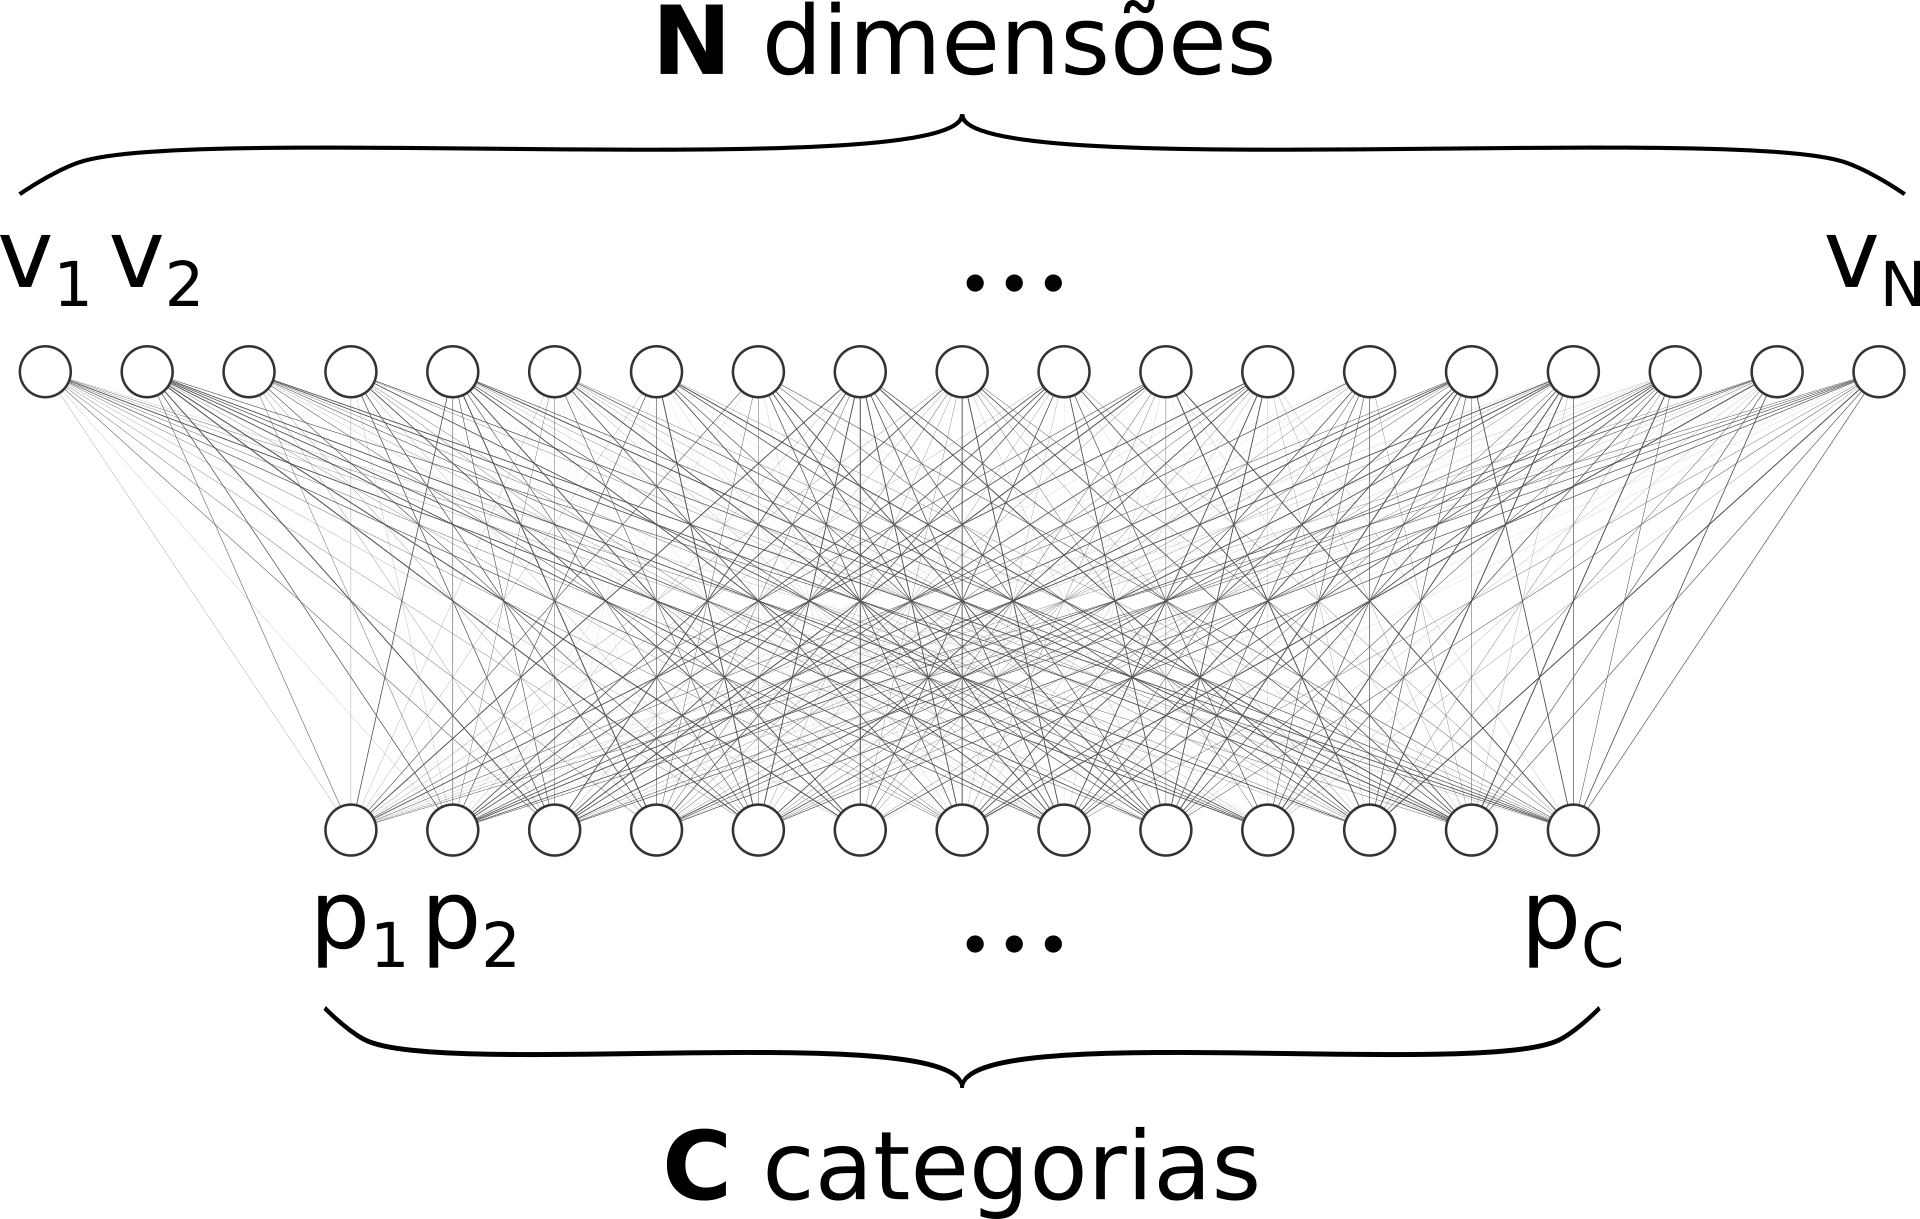
\includegraphics[width=0.6\textwidth]{figures/simple_avg.png}
	\caption{Rede Neural Simples}
	\label{fig:simple_nn}
\end{figure}

A implementação utilizou a linguagem Python e a biblioteca de aprendizado de máquinas Tensorflow, produzindo os resultados indicados na tabela \ref{tab:simple_avg}.

\begin{table}[ht]
\centering
\caption{Métricas da rede neural simples no conjunto de testes para os distintos números de dimensões de \textit{word embedding} analisados}
\vspace{0.5cm}
\begin{tabular}{c|c|c|c|c}
 
Dimensões & Acurácia & F1-Score & Precisão & AUC ROC\\
\hline
50   & 0.7368 & 0.7213 & 0.7239 & 0.9497\\
100  & 0.7641 & 0.7552 & 0.7551 & 0.9583\\
300  & 0.8014 & 0.7940 & 0.7949 & 0.9689\\
600  & 0.8146 & 0.8082 & 0.8094 & 0.9724\\
1000 & \textbf{0.8216} & \textbf{0.8171} & \textbf{0.8183} & \textbf{0.9746}
\end{tabular}
\label{tab:simple_avg}
\end{table}

Apesar de não ser um modelo complexo, um ponto de destaque foi a sua capacidade de generalização, pois não foi observada tendência de \textit{overfitting} conforme ilustra o gráfico da figura \ref{fig:loss_50}.

\begin{figure}[!ht]
	\centering
	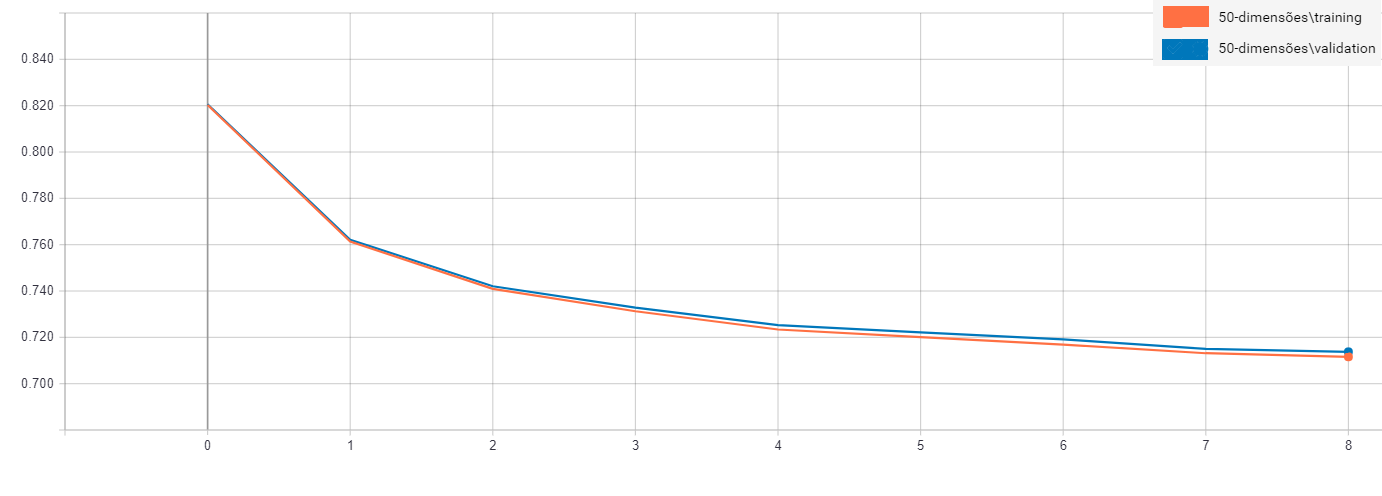
\includegraphics[width=1.1\textwidth]{figures/loss-50.PNG}
	\caption{Curva da função de custo ao término de cada \textit{epoch} de treinamento para 50 dimensões de \textit{word embedding} no modelo rede neural simples}
	\label{fig:loss_50}
\end{figure}

Além disso, como era de se esperar a partir dos resultados listados na tabela \ref{tab:simple_avg}, houve uma boa separação das classes selecionadas nas previsões. Conforme apresenta a figura \ref{fig:confusion_matrix_1000_simpleAvg}, apenas categorias que são difíceis de serem distinguidas até mesmo por seres humanos tiveram um índice de acerto menor do que 83\%. Nesses casos, as classes majoritárias, vide figura \ref{fig:pie_labels_graph}, foram favorecidas.

\begin{figure}[!ht]
	\centering
	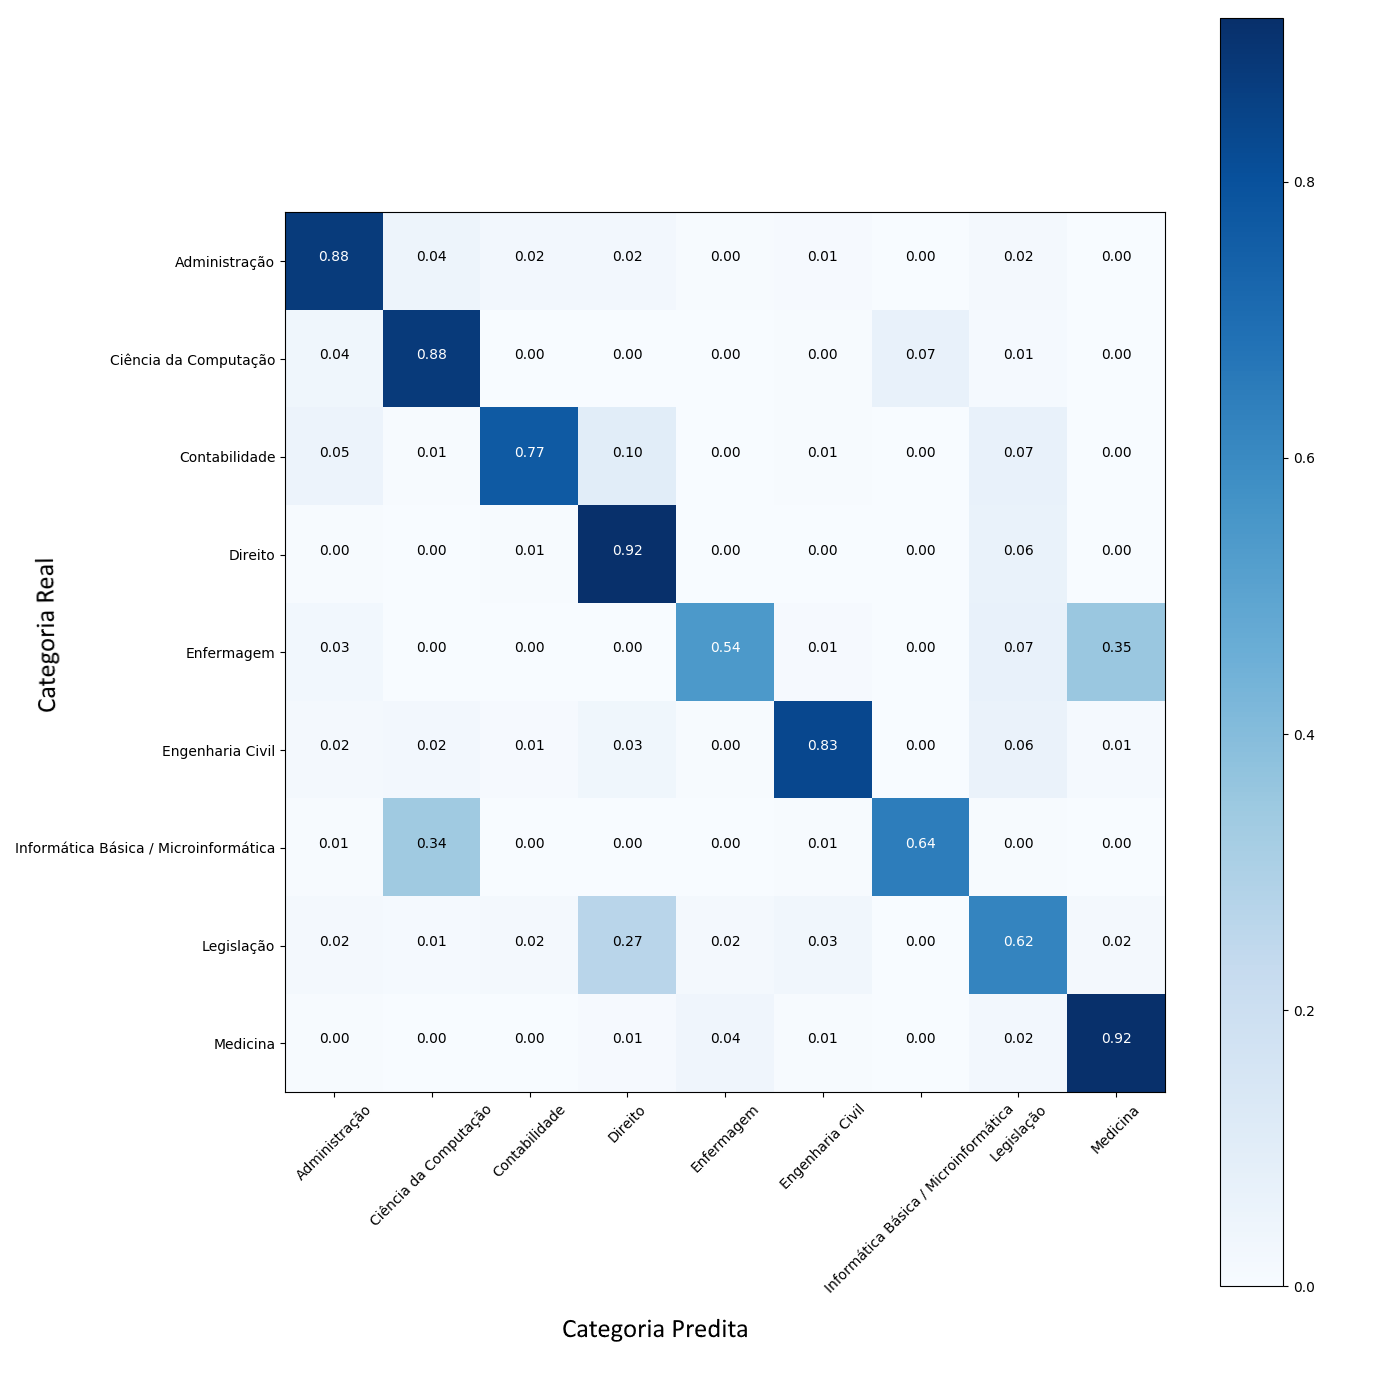
\includegraphics[width=1.1\textwidth]{figures/SimpleAvg_1000_Confusion_matrixnormalized.png}
	\caption{Matriz de confusão normalizada do conjunto de testes com o uso de 1000 dimensões de \textit{word embedding} no modelo rede neural simples}
	\label{fig:confusion_matrix_1000_simpleAvg}
\end{figure}

Contudo, vale ressaltar que esse é um modelo simples de rede neural e não é recomendado para essa aplicação, o seu propósito aqui está diretamente relacionado com a sua simplicidade: atuar como teste inicial de um modelo baseado em \textit{word embedding}, pois, caso existam erros, um primeiro teste com um modelo complexo é mais difícil de ser depurado. 

\section{Vetorização Sequencial}

Além da aglutinação por média da representação numérica de palavras por \textit{embedding}, também se utilizou sequencialmente a representação de cada uma das palavras do texto. Diferentemente das versões exploradas até então, o uso sequencial leva em conta a ordem com que as palavras estão dispostas ao longo do texto para a sua classificação, sendo, portanto, capaz de capturar mais nuâncias do texto.

\subsection{Redes Convolucionais Separáveis}

A implementação SepCNN foi feita utilizando 2 blocos de duas convoluções separáveis cada conforme a figura \ref{fig:sepcnn_overview} e foram utilizados 64 filtros de tamanho 3 \textit{dropout} de 20\%. O modelo SepCNN foi inspirados nos estudos de \cite{DBLP:journals/corr/Chollet16a}.

\begin{figure}[!ht]
	\centering
	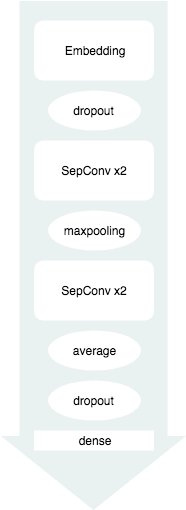
\includegraphics[width=0.3\textwidth]{figures/sepcnn_overview.png}
	\caption{Diagrama sequencial das etapas realizadas na implementação SepCNN}
	\label{fig:sepcnn_overview}
\end{figure}

Cada camada "SepConv x2" é a junção de duas etapas de \textit{depthwise/pointwise} conforme ilustra a figura \ref{fig:sepcnn_detail}.

\begin{figure}[!ht]
	\centering
	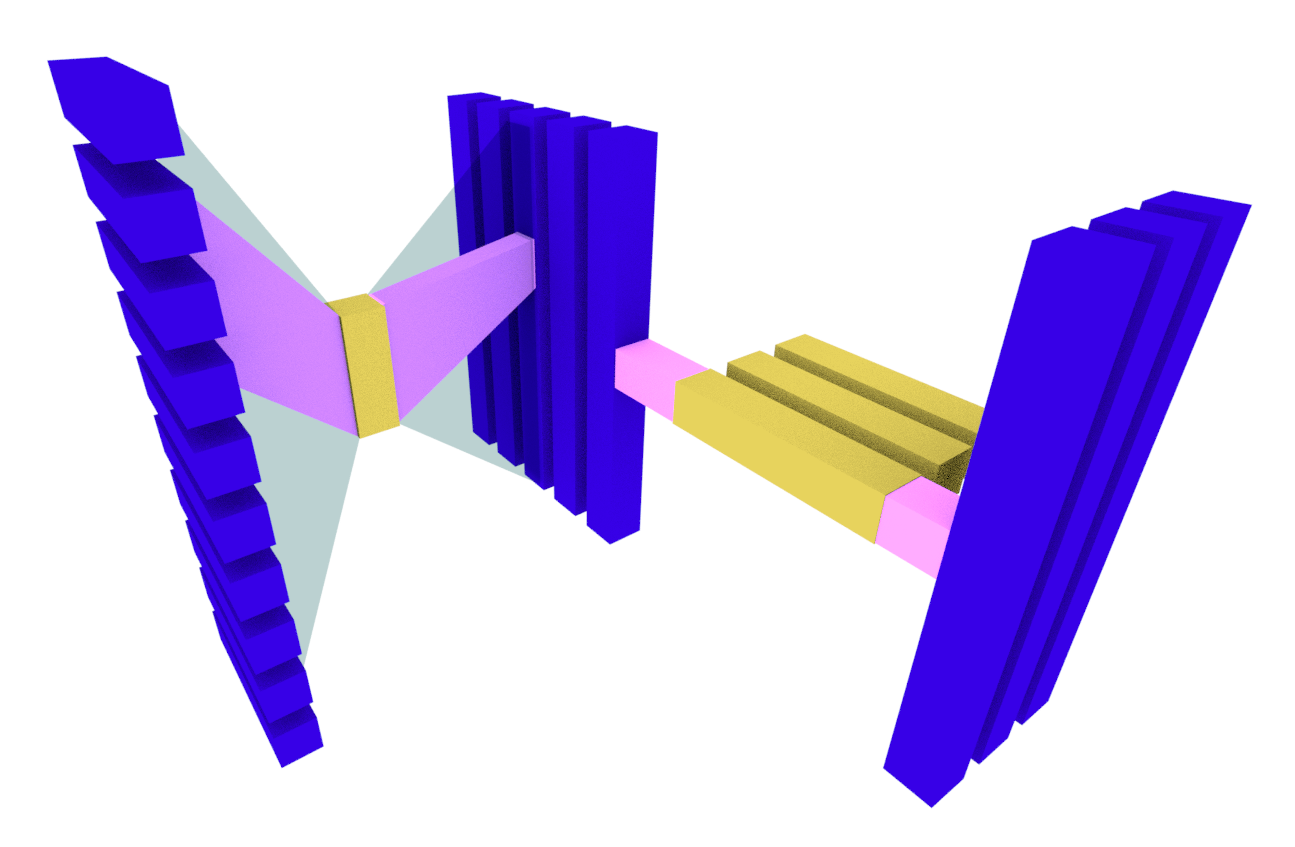
\includegraphics[width=\textwidth]{figures/sepcnn.png}
	\caption{Esquema ilustrativo de convolução separável. Os filtros (em amarelo) representam da esquerda para a direita o \textit{depthwise} e os \textit{pointwise}. Neste exemplo, o cada palavra possui 5 dimensões e cada enunciado 10 palavras. O número de filtros é 3.}
	\label{fig:sepcnn_detail}
\end{figure}

Conforme esperado, o SepCNN apresentou bons resultados de acurácia como pode ser notado na figura \ref{fig:sepcnn_confusion}. Outra vantagem deste modelo foi sua execução mais rápida em treinamento.

\begin{figure}[!ht]
	\centering
	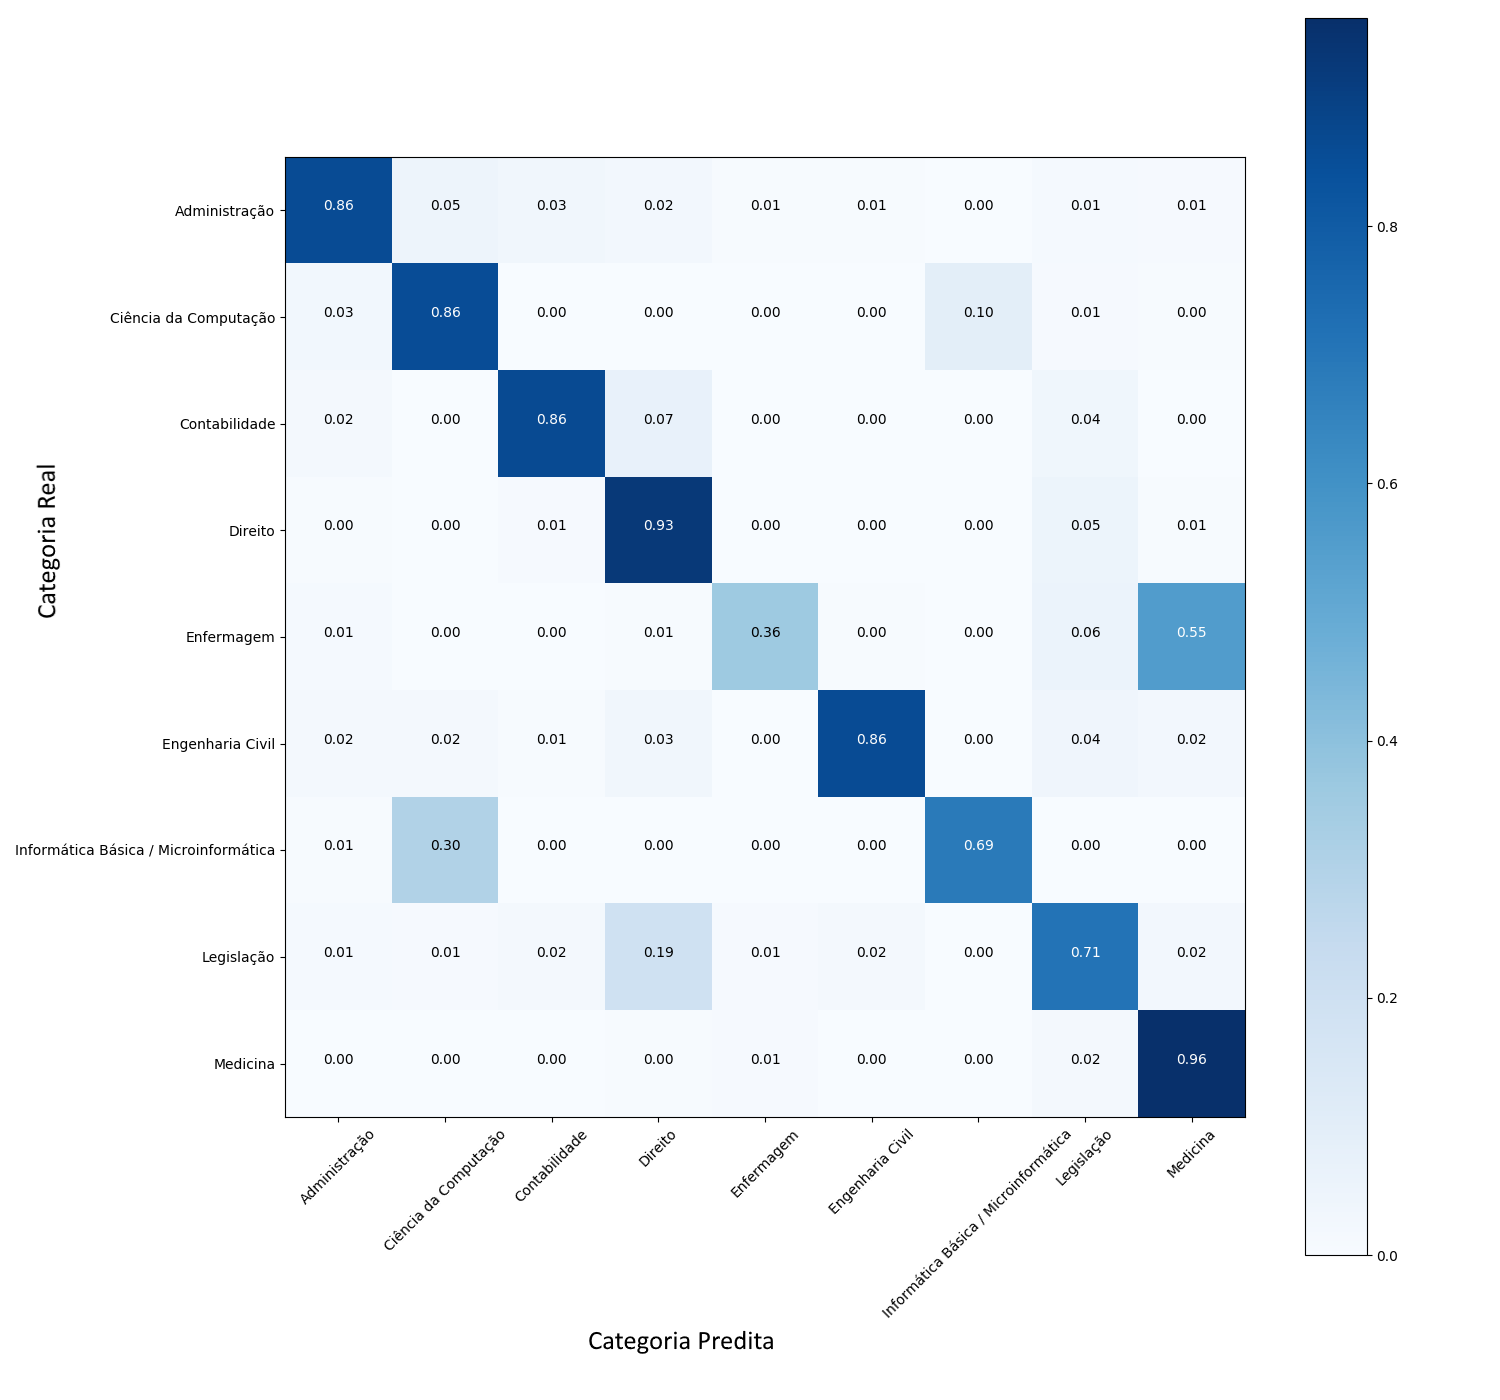
\includegraphics[width=1.1\textwidth]{figures/sepcnn_confusion.png}
	\caption{Matriz de confusão normalizada do modelo SepCNN para 50 dimensões de \textit{embedding}}
	\label{fig:sepcnn_confusion}
\end{figure}

\subsection{RNN simples com células LSTM} \label{section:RNN_simple}

Este modelo se trata da estrutura tradicional de uma rede neural recorrente e possui, como unidade de repetição, uma célula do tipo LSTM conforme ilustra a figura \ref{fig:LSTM}. Nesse modelo, "os neurônios" de memória da célula após o processamento de todas as etapas recorrentes são usados como dados de entrada para uma rede neural simples idêntica ao modelo já descrito e ilustrado pela figura \ref{fig:simple_nn}. A performance dessa rede neural recorrente foi intermediária quando comparada aos outros modelos de redes neurais baseadas em \textit{word embeddings} como pode ser visto em sua matriz de confusão na figura \ref{fig:LSTM_CONF}.

\begin{figure}[!ht]
	\centering
	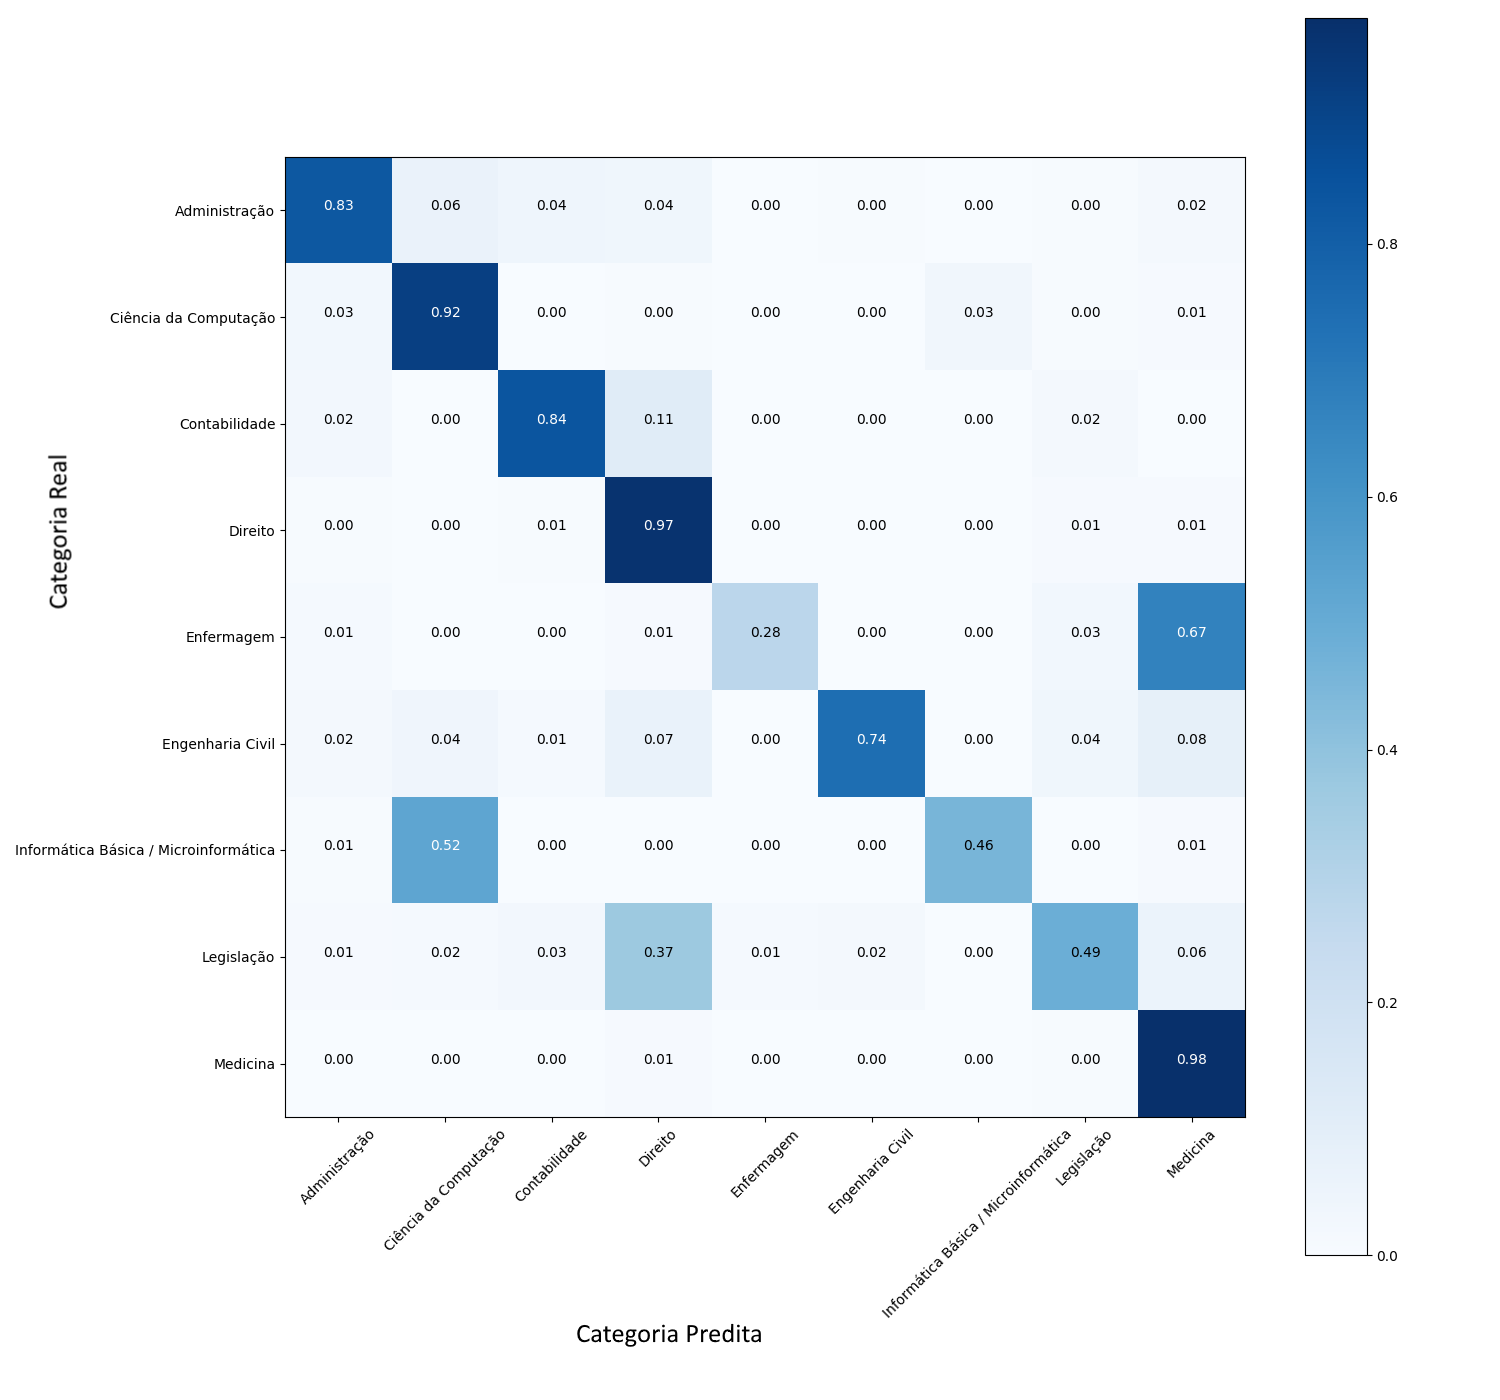
\includegraphics[width=1.0\textwidth]{figures/lstm_confusion.png}
	\caption{Matriz de confusão normalizada do modelo RNN simples com células LSTM e 50 dimensões de \textit{embedding} }
	\label{fig:LSTM_CONF}
\end{figure}

\begin{figure}[!ht]
	\centering
	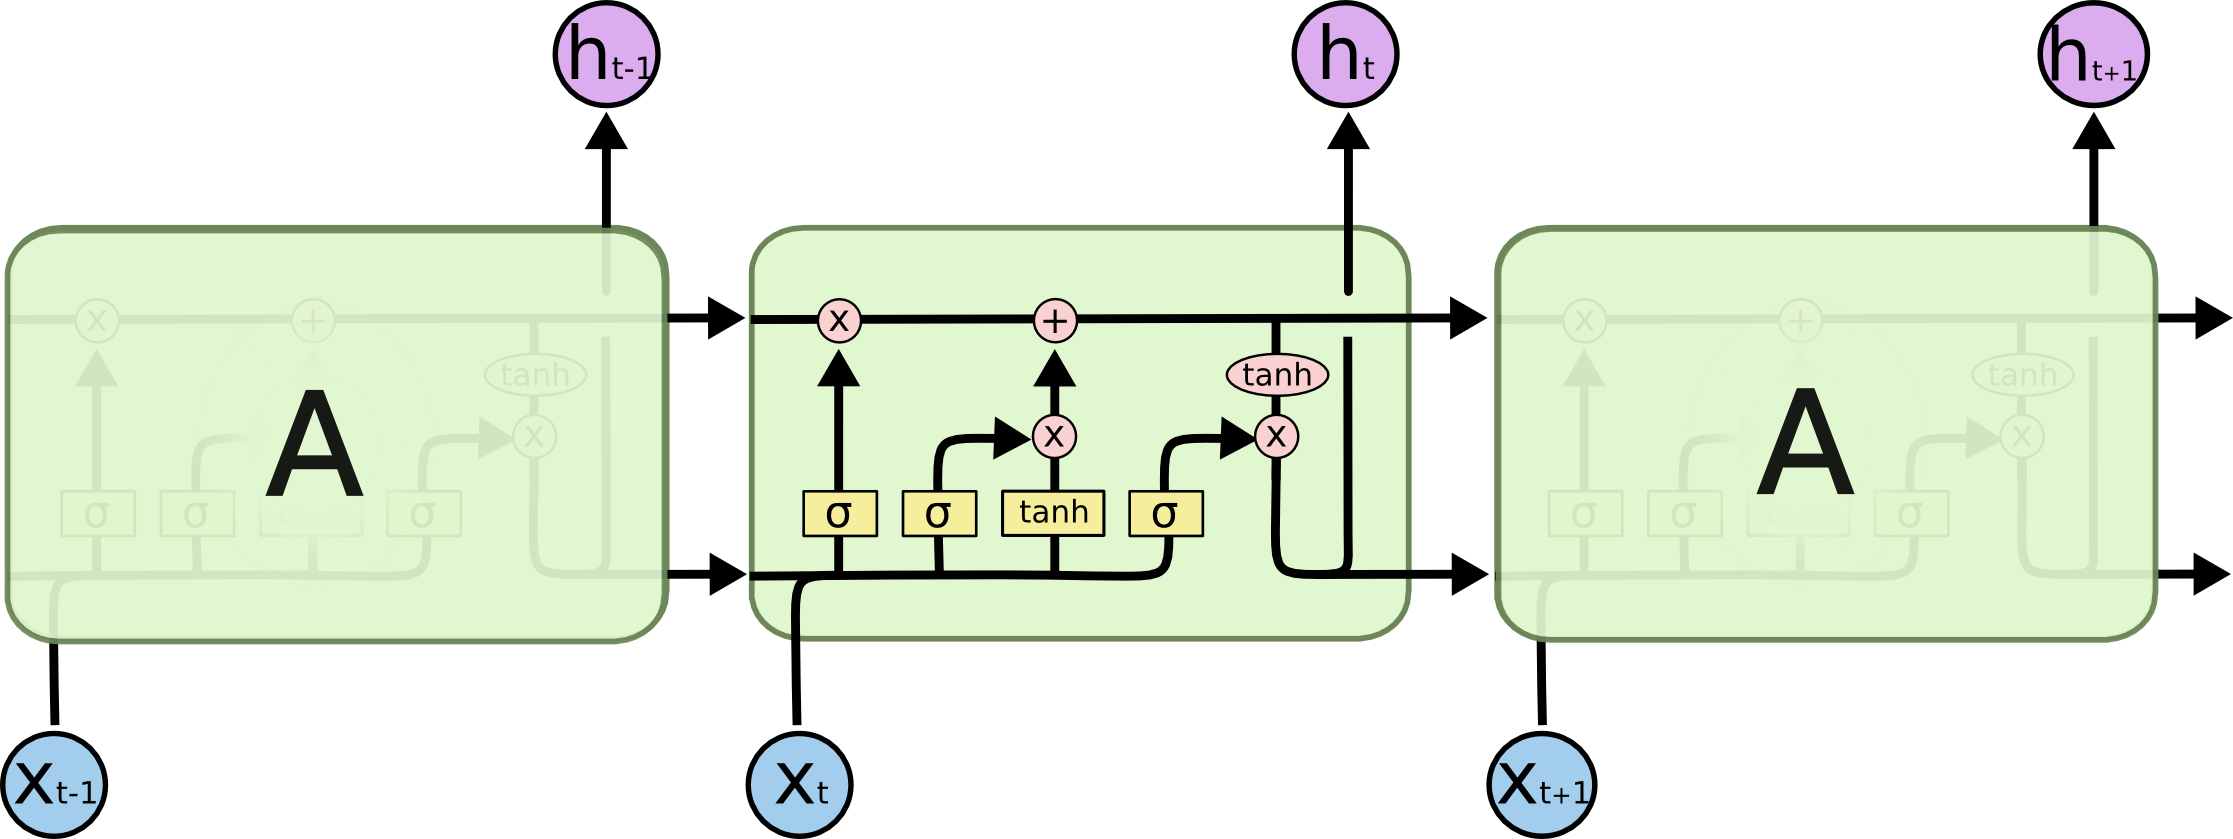
\includegraphics[width=1.0\textwidth]{figures/LSTM3-chain.png}
	\caption{Diagrama esquemático da um LSTM (fonte: \cite{ColahLSTM})}
	\label{fig:LSTM}
\end{figure}

\subsection{\textit{Stacked} RNN com células LSTM}

Uma sofisticação do modelo descrito na seção \ref{section:RNN_simple} é a adição de mais uma camada com uma segunda célula LSTM conforme ilustra a figura \ref{fig:StackedRNN}. Assim, após o processamento de cada entrada
x\textsubscript{t}, a saída correspondente h\textsubscript{t}, conforme a figura \ref{fig:LSTM}, não seria descartada, mas sim repassada para uma camada de \textit{dropout} cujo resultado é usado como entrada para a segunda célula LSTM.

\begin{figure}[!ht]
	\centering
	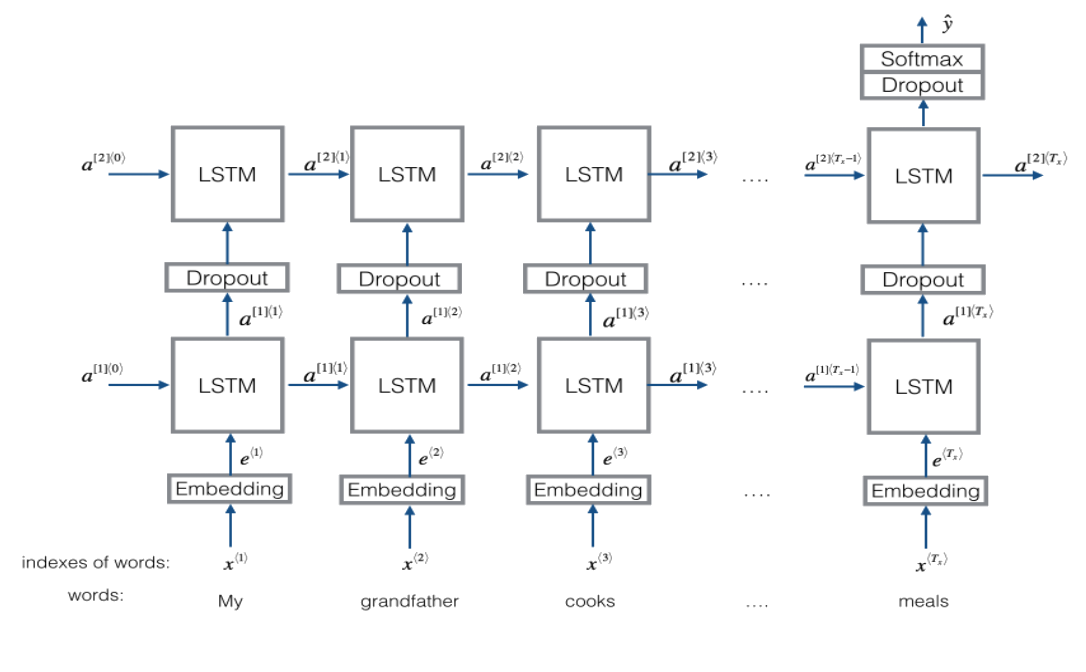
\includegraphics[width=1.0\textwidth]{figures/StackedRNN.png}
	\caption{Diagrama de uma topologia do tipo \textit{stacked} RNN (fonte: Coursera)}
	\label{fig:StackedRNN}
\end{figure}